\documentclass{ReportTemplate}

\title{CSEL}
\author{Macherel Rémy}
\date{\today}
\subtitle{Rapports des TP}
\subsubtitle{}
\location{Fribourg,}
\contact{remy.macherel@master.hes-so.ch}
\version{1.0}



\begin{document}
\maketitlepage

\newpage

\maketableofcontent

\medskip
\chapter{TP 1}
\section{Résumé du travail pratique 1}
Dans ce TP, nous allons mettre en place un environnement de développement afin
de faciliter les développements futures. Cet environnement utilise des container
Docker (Docker-compose) pour assurer la compatibilité entre les différentes
machines. Un container est composé de tous les outils nécessaire à la
cross-compilation et l'autre pour la mise en place d'une partition réseau SAMBA
afin de partager facilement les programmes cross-compilés avec le NanoPi.
\section{Réponses aux questions}
\subsection{Comment faut-il procéder pour générer le U-Boot ?}
On peut regénérer le u-boot uniquement avec la commande : make
uboot-rebuild\newline
See : https://github.com/ARM-software/u-boot/blob/master/Makefile \newline
--> TODO : Ajouter 5-6 lignes qui expliquent ce que fais le make de U-Boot
\subsection{Comment peut-on ajouter et générer un package supplémentaire dans le Buildroot ?}
e ne comprends pas trop le sens de la question mais au sens général, il faut
ajouter le binaire ainsi que des fichiers de configurations (qui définissent par
exemple les dépendances). On peut par exemple importer depuis GitLab
automatiquement un packet, ou encore ajouter des paquet pour le user space ou le
kernel space et tout cela change les étapes a effectuer. Pour plus
d'informations, la section 18 de la
\href{https://buildroot.org/downloads/manual/manual.html#adding-packages}{documentation}.

\subsection{Comment doit-on procéder pour modifier la configuration du noyau Linux ?}
La commande make linux-menuconfig permet de configurer le noyau et on peut
ensuite ajouter/enlever des modules du noyaux et finalement faire make
linux-rebuild afin de reconstruire le noyau.
\newpage
\subsection{Comment faut-il faire pour générer son propre rootfs ?}
Comme c'est Buildroot qui s'occupe de générer le Rootfs, c'est lui qu'il faut
configurer \newline
cd /buildroot \newline
make menuconfig \newline
On peut aussi par exemple modifier le skelette utilisé pour modifier la
structure des dossiers du rootfs. On peut aussi ajouter des
fichiers/scripts/dossiers par défaut dans le rootfs en ajoutant un
rootfs\_overlay
\textit{/buildroot/board/friendlyarm/nanopi-neo-plus2/rootfs\_overlay/}. Ils
seront automatiquement inséré dans le rootfs après chaques générations.

\subsection{Comment faudrait-il procéder pour utiliser la carte eMMC en lieu et place de la carte SD ?}
Il faut commencer par modifier le script de démarrage en modifiant les deux
lignes suivantes. Il faut remplacer le \textbf{0} par le numéro de MMC que l'on
veut : \newline
 fatload mmc \textbf{0} \$kernel\_addr\_r\ Image \newline
 fatload mmc \textbf{0} \$fdt\_addr\_r nanopi-neo-plus2.dtb \newline
On peut avoir des informations sur les mmc disponible en interrompant le U-Boot
et en tappant la commande : \newline
\begin{minted}{shell}
    => mmc list mmc@1c0f000: 0 (SD) mmc@1c10000: 2 mmc@1c11000: 1 
\end{minted}

Il faut ensuite recompiler le script avec la commande make et reflasher la
carte. Enfin il ne faut pas oublier également de charger l'Image et le device
tree depuis la carte SD vers la mmc interne (a faire une seul fois) ainsi que de
modifier le script de démarrage pour utiliser celui que l'on vient de compiler
avec la commande : \newline
\begin{minted}{shell}
    setenv boot_scripts boot.cifs
\end{minted}
 
Finalement, on peut sauvegarder les modifications avec la commande :\newline
\begin{minted}{shell}
    saveenv
\end{minted}
\subsection{Dans le support de cours, on trouve différentes configurations de l’environnement de développement. Qu’elle serait la configuration optimale pour le développement uniquement d’applications en espace utilisateur ?}
Si on développe uniquement dans le userspace, on pourrait imaginer que l'on
flash la eMMC comme décrit à la question précédente pour s'affranchir de carte
SD et qu'on développe sur notre ordinateur. Pour le partage des programmes une
partition NFS ou la partition CIFS sont très bien et permettent de rendre
transparent le transfert des programmes.
\newpage
\section{Synthèse des connaissances acquises}
\subsection{Non acquis}
Aucune
\subsection{Acquis, mais à exercer}
Les Makefile, debugging (GDB/HDB Server), Principe CIFS
\subsection{Parfaitement acquis}
Le reste comme par exemple ce qui est commande, connexion, Linux (déjà
globalement vu dans un cours précédent)
\section{Infos utiles à retenir}
Pour monter automatiquement un disque réseau cifs : \newline
\begin{minted}[fontsize=\tiny]{shell}
echo "//<server_ip>/workspace /workspace cifs username=<username>,
password=<password>,port=1445,noserverino" >> /etc/fstab
\end{minted}
Lorsqu'on créer une nouvelle partition, il faut l'aligner sur 2048 bits. On peut
calculer le début de la prochaine partition par rapport à la précédente comme
ceci : \newline
<prev\_end\_sector> + (2048 - <prev\_end\_sector>  \% 2048)
\section{Feedback global}
Dans l'ensemble laboratoire très intéressant et bon point de départ pour un
cours comme celui-ci. Assez dirigé pour nous indiquer la bonne voie mais pas
trop pour qu'on puisse tester des choses. Nous aurions bien souhaité un peu plus
de maitère sur les Makefiles.\newline
Nous avons également pour le flash de la carte SD développé un script permettant
ceci de manière automatique (à voir dans le dossier script le FlashSDCard.sh).
Ce script permet donc le flash de la SD Card avec les fichiers nécessaires sans
utiliser le logiciel \textit{Balena}. Afin de l'utiliser, il suffirait de
modifier le chemin d'accès à l'image (ligne 2 du script). Il a également été
très intéressant de découvrir les differentes méthodes de debugging possibles
lors du développement de systèmes embarqués. Parmis celles vues en cours, nous
avons particulièrement testé la méthode utilisant GDB / GDB Server. La capacité
de cette méthode à réaliser du débugging à distance était pour nous un point
fort. Cette méthode permettait entre autres d'exécuter le code présent sur la
cible pas à pas et de découvrir de potentielles erreurs.\newline
\subsection{Problèmes rencontrés}
Pour un des membres du groupe, une fois le CIFS mis en place, le nanoPi était
incapable de démarrer et semblait relancer sa séquence de boot indéfiniment.
Nous avons par la suite déterminé que ceci était dû à une trop faible
alimentation via un HUB USB qui faisait que lorsque le nanoPi tentait de se
connecter via le réseau la tension n'était pas suffisante et celui-ci
s'éteignait puis rebootait directement.

\chapter{TP 2}
\section{Résumé du laboratoire}
Ce laboratoire concerne les modules noyaux. Il est très important et utile afin
de mettre en pratique la manière vue durant les cours sur ces modules. Il permet
de parcourir les différentes possibilités de ces modules comme par exemple:
\begin{itemize}
    \item Modules out of tree
    \item Gestion de la mémoire
    \item Accès I/O
    \item Threads dans le noyau
    \item Mise en sommeil (relatif aux threads)
    \item Interruptions
\end{itemize}
Durant les différents exercices de ce travail pratique nous avons parcouru ces
possibilités et implémenté chacune d'entre elles. Les fichiers sources se trouve
dans le dossier csel-workspace/src/02\_module/exercice..\newline

\section{Réponses aux questions}
\subsection{Trouvez la signification des 4 valeurs affichées lorsque l’on tape la commande cat /proc/sys/kernel/printk}
\label{sec:signification}
Cela affiche les console\_loglevel (niveaux de logs de la console) actuels, dans
notre cas sur le nanopi les valeurs affichées sont 7 4 1 7, comme le montre la
\href{https://www.kernel.org/doc/html/latest/core-api/printk-basics.html}{documentation}
l'ordre des chiffres correspond à : 
\begin{enumerate}
    \item current
    \item default
    \item minimum
    \item boot-time default
\end{enumerate}

\begin{figure}[H]
    \centering
    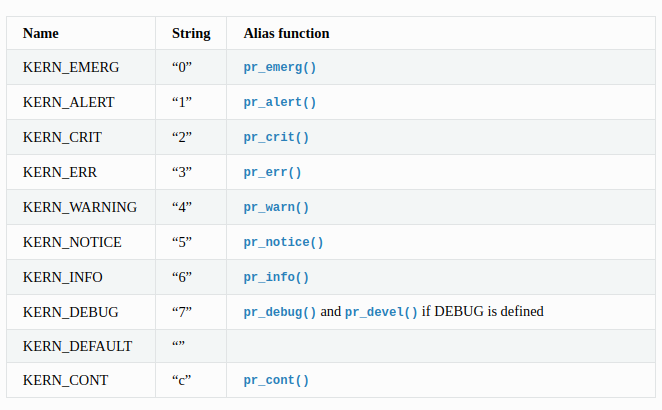
\includegraphics[width=0.7\textwidth]{imageSources/console_loglevels.png}
    \caption{Console log levels correspondance}
    \label{fig:LogLevels}
\end{figure}
\section{Synthèse des connaissances acquises}
\subsection{Non acquis}

\subsection{Acquis, mais à exercer}

\subsection{Parfaitement acquis}
\section{Feedback exercices}
\subsection{Exercice 01}
L'exercice 01 ne nous a globalement pas posé de problèmes, nous avons suivi les
slides du cours afin de créer le skeleton.c ainsi que son makefile. Nous l'avons
ensuite compilé puis chargé dans le nanoPi. Nous avons ensuite effectué la
commande \textit{dmesg} afin de vérifier que le noyau a bien été chargé en
affichant les \textit{printk} du code.
\subsection{Exercice 02}
Dans cet exercice, il suffisait d'adapter le module pour qu'il puisse recevoir
des paramètres, pour ce faire, nous avons ajouté comme les lignes de la figure
suivante à la suite des include.
\begin{figure}[H]
    \centering
    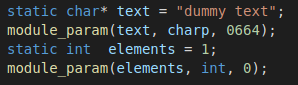
\includegraphics[width=0.7\textwidth]{imageSources/ModuleParams.png}
    \caption{Add modules parameters}
    \label{fig:ModuleParams}
\end{figure}
Nous avons suivi la démarche décrite dans le cours. Les paramètres se
définissent donc de la manière suivante dans la fonction \textit{moduleparam}: \newline
nom de la variable, type de la variable, permissions du fichier correspondant
dans le sysfs. Il serait aussi possible d'ajouter une description au paramètre
en utilisant la macro \textit{MODULE\_PARAM\_DESC(nomVariable,'description')}. Les
informations concernant ceci se trouvent dans le cours ainsi que sur
\href{https://linuxkernel51.blogspot.com/2011/03/use-of-module-parameters-in-kernel.html}{ce
site}.
\newpage
\subsection{Exercice 3}
Voir \ref{sec:signification}.
\subsection{Exercice 4}
L'exercice 4 consistait à définir en paramètre du module un nombre d'élément à
créer ainsi qu'un texte à créer dans ces éléments. Nous avons créé une structure
\textit{elem} contenant le text ainsi qu'un identifiant et un pointeur vers
l'élément suivant. Dans la fonction d'initialisation du module on se charge de
créer un nombre d'éléments égal au paramètre transmis. Ensuite dans la méthode
de sortie du module nous utilisons \textit{kfree} afin de libérer la mémoire
allouée pour chaque élement.
\subsection{Exercice 5}
Dans cet exercice il s'agissait de développer un module noyau permettant
d'afficher diverses informations sur le processeur. Il 'sagissait d'utiliser les
fonctions \textit{request\_mem\_region} afin de demander une région mémoire.
Nous nous sommes tout d'abord interrogés sur le nombre de bytes à réserver puis
après discussion avec le professeur nous avons décidà de réserver l'entièreté de
la page (soit 0x1000). Nous avons également remarqué que la plupart du temps
cette fonction se retrouvait avec un code d'erreur (0) à sa sortie. Cela est
certainement dû au fait que des informations telles que la température ou la MAC
adress sont certainement souvent requises par d'autres processus et donc déjà
réservées. Nous avons ensuite utilisé \textit{ioremap} afin de mapper dans la
mémoire virtuelle les adresses physiques requises pour que l'on puisse ensuite
lire les valeurs nécessaires.
\subsection{Exercice 6}
Rien de spécial à signaler dans cet exercice. Il s'agissait d'instantier un
thread qui affiche un message toutes les 5s.
\subsection{Exercice 7}
Nous avons initialement dans l'exercice 7 peiné à utiliser les fonctions
wait\_event\_interruptible et wake\_up\_interruptible. Nous avions tout d'abord
pensé qu'il n'était pas nécessaire d'utiliser un verrou atomique car nous
pensions que la fonction wake\_up\_interruptible générait le signal permettant
de réveiller le wait, cependant il s'est avéré que ce n'était pas le cas et nous
avons donc dû (comme dans la solution fournie) implémenter un verrou permettant
de bloquer et de signaler au wait que celui-ci doit se réveiller et afficher son
message. Nous avons donc conclus que la queue était présente pour que le thread
se mette en attente si la condition est fausse. Dans notre cas, comme au début
nous avions mis une condition à true en permanence cela tournait dans une boucle
infinie car le fait que la condition soit vraie lui permettait de toujours
passer par dessus la queue. Le wake\_up sert donc juste à indiquer au wait qu'il
doit re-vérifier sa condition. Ces informations furent découvertes en faisant
des tests ainsi qu'en discutant lors de la séance de laboratoire.\newline
\newpage
\subsection{Exercice 8}

\chapter{TP 3}
\section{Résumé du laboratoire}
\section{Réponses aux questions}
\section{Synthèse des connaissances acquises}
\subsection{Non acquis}

\subsection{Acquis, mais à exercer}

\subsection{Parfaitement acquis}
\section{Feedback}
\subsection{Exercice 01}
Les pilotes orientés mémoire permettent d'accéder directement aux
registres en programmant la MMU sans avoir besoin de créer un module noyau.
Pour cet exercice il s'agissait de créer un pilote orienté mémoire afin de
permettre de lire le Chip-ID du processeur. Nous n'avons pas rencontré de
problème particulier dans la réalisation de cet exercice.
\subsection{Exercice 02}
Afin de stocker dans une variable globale du pilote des données reçues par les
commandes echo (write) et cat (read) nous avons implémenté un pilote orienté
caractère. Pour ce faire il fallait (comme démontré dans les slides du cours)
implémenter les différentes \textit{file operations} que sont
read,write,open,release afin que celles-ci permettent les opérations demandées
dans la consigne. Une fois ceci fait, la démarche veut que l'on place dans une
structure de type \textit{file\_operations} ces différentes opérations comme le
montre la figure suivante :
\begin{figure}[H]
    \centering
    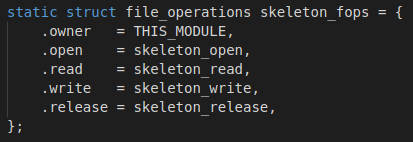
\includegraphics[width=0.7\textwidth]{imageSources/Fops.png}
    \caption{File operations structure}
    \label{fig:Fops}
\end{figure}
Une fois ces operations implémentées, il faut, dans l'initialisation du module,
utiliser \textit{alloc\_chrdev\_region} afin d'allouer un espace pour notre
device. Si cette allocation se passe correctement, on peut utiliser
\textit{cdev\_init} afin d'initialiser le device avec ses file operations. Ces
opérations permettent de définir les opérations supportées par notre
pilote.\newline
A la destruction (exit) du device, on peut supprimer celui-ci à l'aide de
\textit{cdev\_del} et désallouer la mémoire avec
\textit{unregister\_chrdev\_region}. \newline
Lorsque le code est écrit il suffisait de le compiler a l'aide la commande \textit{make},
puis sur la cible utiliser
\begin{minted}{shell} 
    insmod mymodle.ko #(si pas d'arguments) ou 
    insmod mymodule.ko <argName1>=<value1> <argName2>=<value2> #(si arguments)
\end{minted}    
afin de charger le device. Dans notre cas, nous n'avions pas print le major number dans
les fonctions d'initialisation du device et donc afin de retrouver celui-ci nous
avons utilisé la commande 
\begin{minted}{shell}
    cat /proc/devices 
\end{minted}
pour le retrouver. Une fois le major number connu, nous avons effectué la
commande
\begin{minted}{shell}
    mknod /dev/mymodule c 511 0
\end{minted}
afin de créer un node pour le device. Une fois ceci fait il suffisait de tester
l'écriture et la lecture avec par exemple
\begin{minted}{shell}
    echo "salut" > /dev/mymodule #(pour écrire)
    cat /dev/mymodule #(pour lire)
\end{minted} 
Une fois que le node est créé, on peut lister le major/minor avec la commande 
\begin{figure}[H]
    \centering
    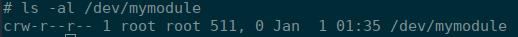
\includegraphics[width=0.7\textwidth]{imageSources/MajorMinor.png}
    \caption{Major and Minor number}
    \label{fig:MajorMinor}
\end{figure}
\newpage
\subsection{Exercice 03}
L'exercice 03 est une adaptation de l'exercice 2 afin de pouvoir définir par
paramètre (par défaut 3) le nombre de devices pouvant être créés. Afin de tester
ce fonctionnement nous avons tout d'abord adapté le code (voir code source),
puis nous avons essayé de créer 4 nodes (commande \textit{mknode} avec 4 minor
number différents). La création s'est effectuée mais lorsque l'on souhaite lire
ou écrire dans le 4ème node cela ne marche pas. Cela est logique car le nombre
de noeuds est limité à 3. Exemple :
\begin{figure}[H]
    \centering
    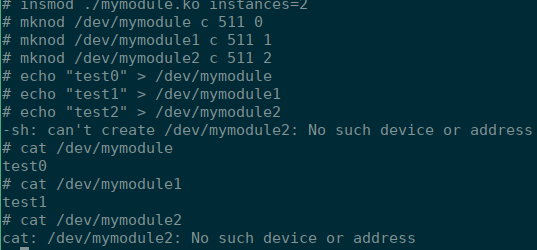
\includegraphics[width=0.7\textwidth]{imageSources/Ex3_cDev.png}
    \caption{Exercice 03 tests}
    \label{fig:Ex3Tests}
\end{figure}
\subsection{Exercice 04}
Nous n'avons pas spécialement eu de difficultés à réaliser ces exercices mais
ceci nous a permis de tester l'écriture dans un character device et de voir que
l'on peut écrire jusqu'à ce que le buffer soit plein (le retour est -EIO). Une
fois que celui-ci est plein, le programme casse la boucle et on va lire le
contenu du device.
\subsection{Exercice 05}

\subsection{Exercice 07}

\end{document}


